\documentclass[10pt]{beamer}
\usepackage{etex}
\usepackage{subfig}
\usepackage[english]{babel}
\usepackage[utf8]{inputenc}
\usepackage[T1]{fontenc}
\usepackage{lmodern}

% AMSLaTeX packages
\usepackage{amsthm,amsmath,amsfonts}
\usepackage[algoruled]{algorithm2e}

\usetheme{default}
\useoutertheme{default}
% we want to use images
\usepackage{graphicx,hyperref,grffile}

% table relates packages
\usepackage{booktabs,multirow}
\usepackage{realboxes}

\usepackage{xcolor}
\usepackage{adjustbox}
\usepackage{ulem}
%\usepackage{subfigure}
%\usepackage[numbers]{natbib}
%\usepackage{natbib}
\usepackage[style=authortitle]{biblatex}
\addbibresource{presentation.bib}
% \setbeamercolor{bibliography entry note}{fg=red}
%\usepackage{todonotes}
%\presetkeys{todonotes}{inline}{}
%\usepackage{multimedia}
%\usepackage{bibentry}
%\nobibliography*
%\let\labelindent\relax
%\usepackage{enumitem}
%\usepackage{pst-grad} % For gradients
%\usepackage{pst-plot}
%\usepackage{pstricks-add}
\usepackage[off]{pstricks,auto-pst-pdf} % when switched to on, don't forget to include
                               % the aforementioned pstricks packages.

% Changes the color of bullets and other fonts to match the NormalANLBlue template
\definecolor{anlpresentationblue}{RGB}{127 160 195}
\setbeamercolor{structure}{fg=anlpresentationblue!150} % for slide titles, etc
\setbeamercolor{block title}{fg=white,bg=anlpresentationblue} % For blocks
\setbeamercolor{block body}{fg=black,bg=anlpresentationblue!20} % For blocks

% Force revisiting of table of contents every time a new section is declared
\AtBeginSection[]
{
   \begin{frame}
       \frametitle{Outline}
       \tableofcontents[currentsection]
   \end{frame}
}

\setlength\arraycolsep{1.4pt}% some length
\definecolor{darkgreen}{HTML}{3C8031}
%\definecolor{darkgreen}{HTML}{2D2F92}
%\definecolor{darkgreen}{HTML}{F58137}
\newcommand{\vect}[1]{\boldsymbol{#1}}

%gets rid of navigation symbols
\setbeamertemplate{navigation symbols}{}
\setbeamertemplate{itemize items}[circle]

%gets rid of bottom navigation bars
\setbeamertemplate{footline}[page number]{}
\setbeamertemplate{headline}{}
\hypersetup{
    colorlinks=true,
    citecolor = blue
}
%<your other options\dots>,

%\usepackage{cmbright} % A font that I like
% \usepackage[T1]{fontenc}

% \renewcommand{\seriesdefault}{sb} % Changes the font to semibold

\usebackgroundtemplate{
\includegraphics[width=\paperwidth]{NormalANLBlue}}

\title[]{
Solving Power Flow on GPUs in Julia \\
}
\author[]{Michel Schanen*, Daniel Adrian Maldonado, Mihai Anitescu}
\subtitle{}
\institute[ANL/MCS]{Argonne National Laboratory\\ Mathematics and Computer Science
Division}
\date{Jul 15, 2020}

\usepackage{tikz,tikz-cd}
\usepackage{pgfplots,pgfplotstable}
\usetikzlibrary{pgfplots.groupplots}
\usetikzlibrary{positioning}
\usetikzlibrary[shapes,arrows,trees]
\usetikzlibrary{matrix,decorations.pathmorphing}
% \usepackage{epstopdf}
\usepackage{tensor}
\usepackage[usecolors=true, usebox=true, charsperline=65]{jlcode}
\addtobeamertemplate{footnote}{}{ \vspace{2ex}}

\newcommand{\Var}[1]{\mathrm{Var}\left \{ #1\right\}} % Variance
\newcommand{\vol}[1] {\operatorname{vol}\left( #1 \right)}
\newcommand{\E}[1]{\operatorname{\mathbb{E}}\left[ #1\right]} % Expected value
\renewcommand{\P}[1]{\operatorname{\mathbb{P}}\left[ #1\right]} % Expected value
\newcommand{\norm}[1]{\left\| {#1} \right\|}
\newcommand{\argmax}{\operatornamewithlimits{arg\,max}}
\newcommand{\argmin}{\operatornamewithlimits{arg\,min}}
\newcommand{\jeffa}{\phantom{\sum_{i = 1}^{m}\tilde{f}\mathcal{N}(0,\sigma^2)}}
\newtheorem{proposition}[theorem]{Proposition}
\newcommand\Perms[2]{\tensor[_{#1}]P{_{#2}}}
\newcommand{\minimize}{\operatornamewithlimits{minimize}}
\newcommand{\tu}[1]{\textup{#1}}
\newtheorem{assumption}[theorem]{Assumption}
%\newcommand{\adj}[1]{{#1_{(1)}}}
%\newcommand{\tlm}[1]{{#1^{(1)}}}
\newcommand{\adj}[1]{\bar{#1}}
\newcommand{\tlm}[1]{\dot{#1}}
%\newcommand{\tlm}[1]{{#1^{(1)}}}
% \setbeameroption{show notes}
% \setbeameroption{show only notes}
\newcommand{\mynode}[2]{%
%\pspolygon(#1,#2)(#3,#4)(! 0.5 dup add #1 sub #2)(! #3 #2 dup add #4 sub)
%\psframe(! 0.5 0.5 add #1 sub 1 1 add)(1 ,6)
\psframe(! #1 0.5  sub #2 0.5 sub)(! #1 0.5  add #2 0.5 add)
%\psline(! #1 0.5 sub #2)(! #1 0.5 add #2)
%\rput(! #1 -0.25 #2 add){CPU}
%\rput(! #1 0.25 #2 add){Mem.}
}

% Some macros for Taylor series
\newcommand{\sumone}[1]{\ensuremath{\sum_{#1 = 1}^n}}
\newcommand{\sumtwo}[2]{\ensuremath{\sum_{#1,#2 = 1}^n}}
\newcommand{\sumthree}[3]{\ensuremath{\sum_{#1,#2,#3 = 1}^n}}
\newcommand{\sumfour}[4]{\ensuremath{\sum_{#1,#2,#3,#4 = 1}^n}}
\newcommand{\D}[0]{\mathrm{D}}

\newcommand{\partone}[2]{\D_{#2} g_{#1}}
%\newcommand{\parttwo}[3]{H^{#1}_{#2#3}}
\newcommand{\parttwo}[3]{\D^2_{#2 #3} g_{#1}}
%\newcommand{\partthree}[4]{T^{#1}_{#2#3#4}}
\newcommand{\partthree}[4]{\D^3_{#2 #3 #4} g_{#1}}
\newcommand{\bigo}[1]{\mathcal{O}\left( #1 \right)}
%\newcommand{\vect}[1]{\boldsymbol{#1}}
%\newcommand{\E}[1]{\mathbb{E}\left[ #1 \right]}

\usepackage{array}
\newcolumntype{x}[1]{>{\centering\arraybackslash\hspace{0pt}}p{#1}}
\setbeameroption{hide notes}

\begin{document}
\setbeamertemplate{footline}{}
{
\usebackgroundtemplate{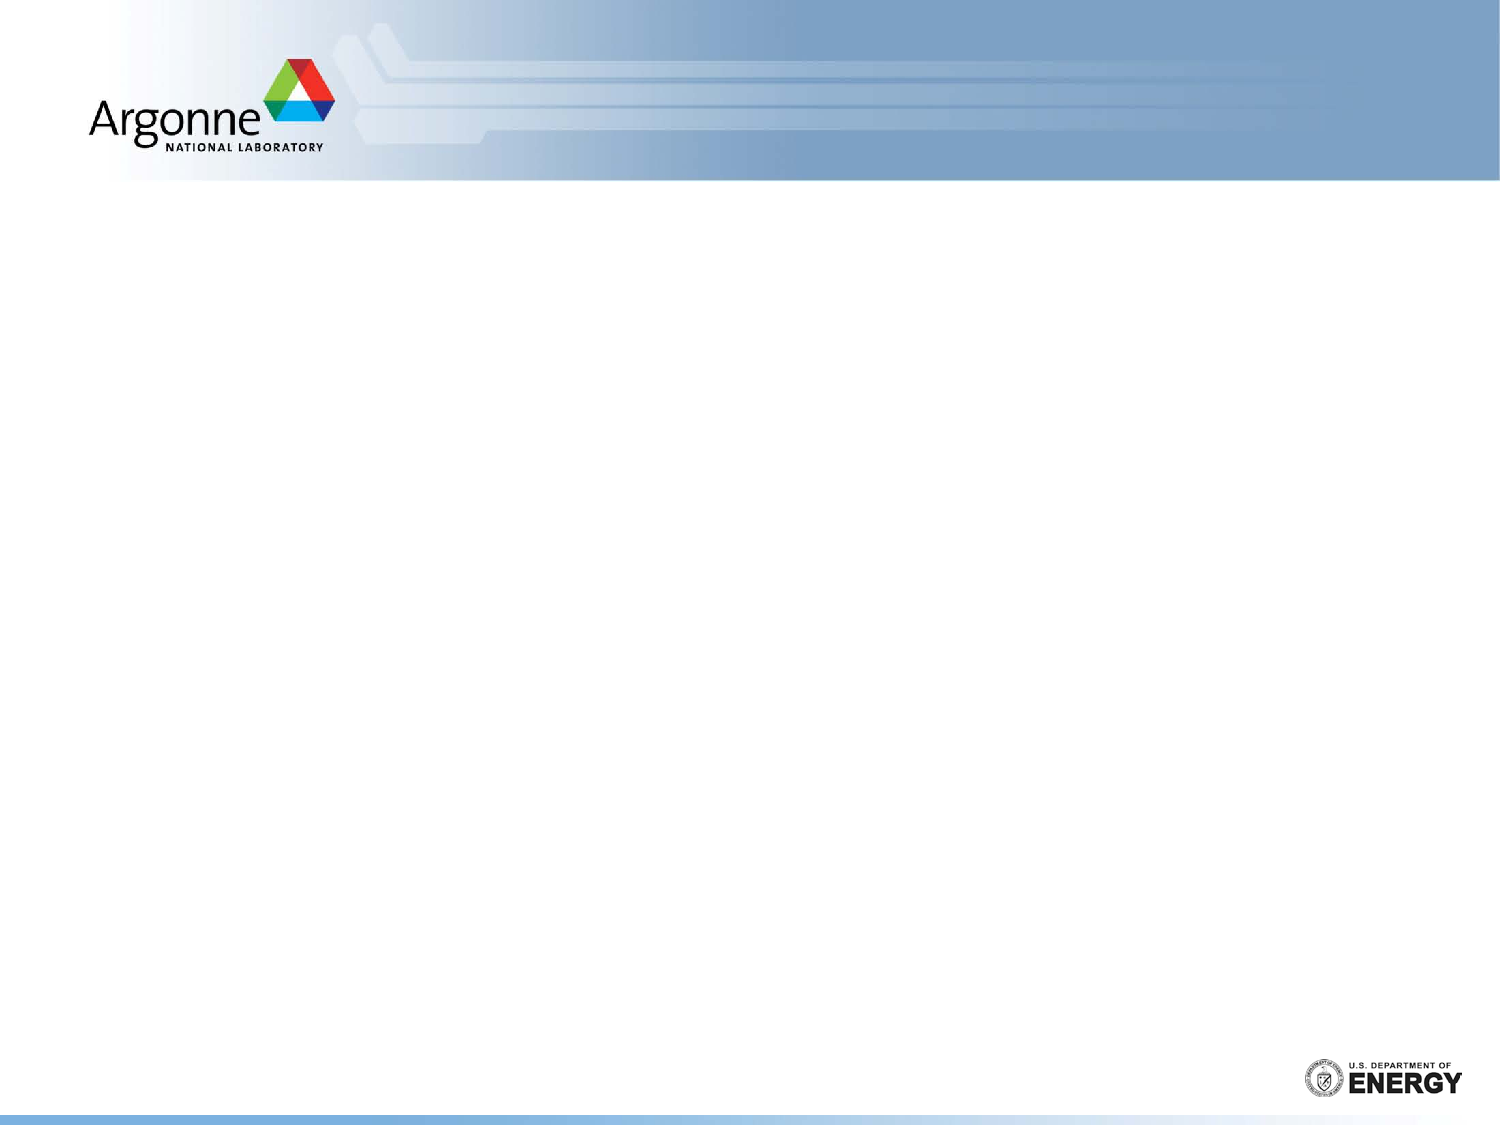
\includegraphics[width=\paperwidth]{TitleANLBlue}}
\frame{\titlepage}
}

% \setbeamertemplate{footline}[]{\insertframenumber of \inserttotalframenumber}
\setbeamertemplate{footline}{
  \begin{beamercolorbox}{footlinecolor}
    \hfill
    \begin{minipage}[c]{3cm}
        \tiny{{\color{anlpresentationblue} \hfill \insertframenumber{} of \inserttotalframenumber} }
    \end{minipage}      
    \begin{minipage}[c]{10cm}
       {\color{white} .}
    \end{minipage}      
   \end{beamercolorbox}
}

% DO NOT COMPILE THIS FILE DIRECTLY!
% This is included by the other .tex files.
\begin{frame}
  \frametitle{Upcoming Supercomputers}
    \begin{center}
      
\includegraphics[width=.25\textwidth]{./figures/ecp} \\
      % \includegraphics[width=.75\textwidth]{./figures/go} 
    \end{center}
  \begin{columns}[T]
    \begin{column}{0.49\textwidth}
      \begin{center}
        {\bf Aurora}\\
        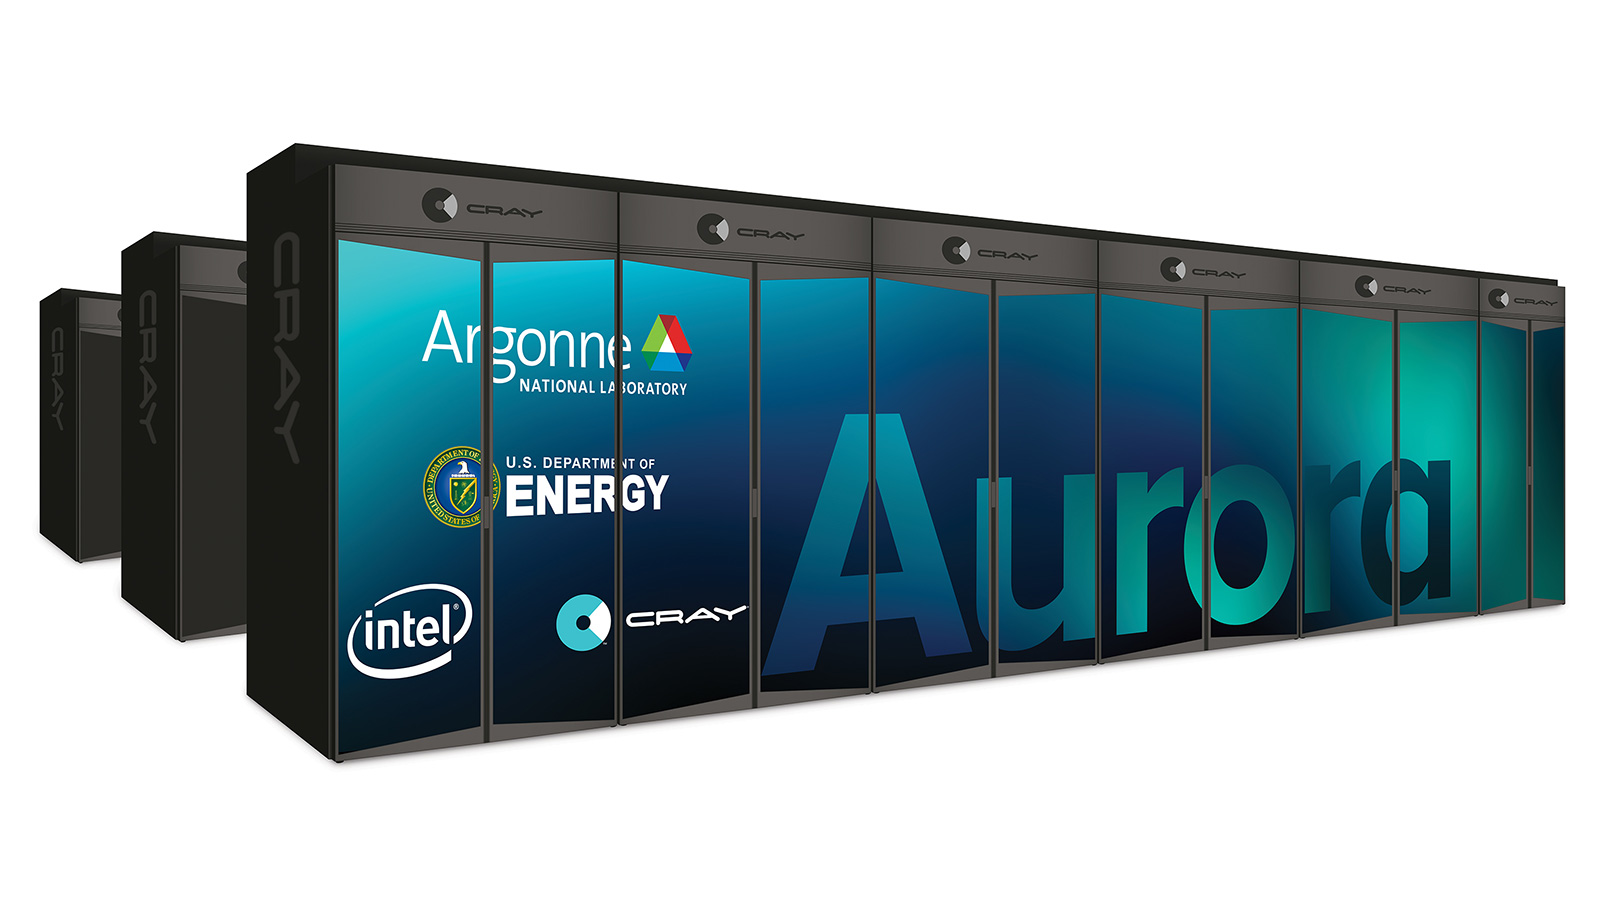
\includegraphics[width=0.75\textwidth]{./figures/aurora}
      \end{center}
    \end{column}
    \begin{column}{0.49\textwidth}
      \begin{center}
        {\bf Frontier}\\
        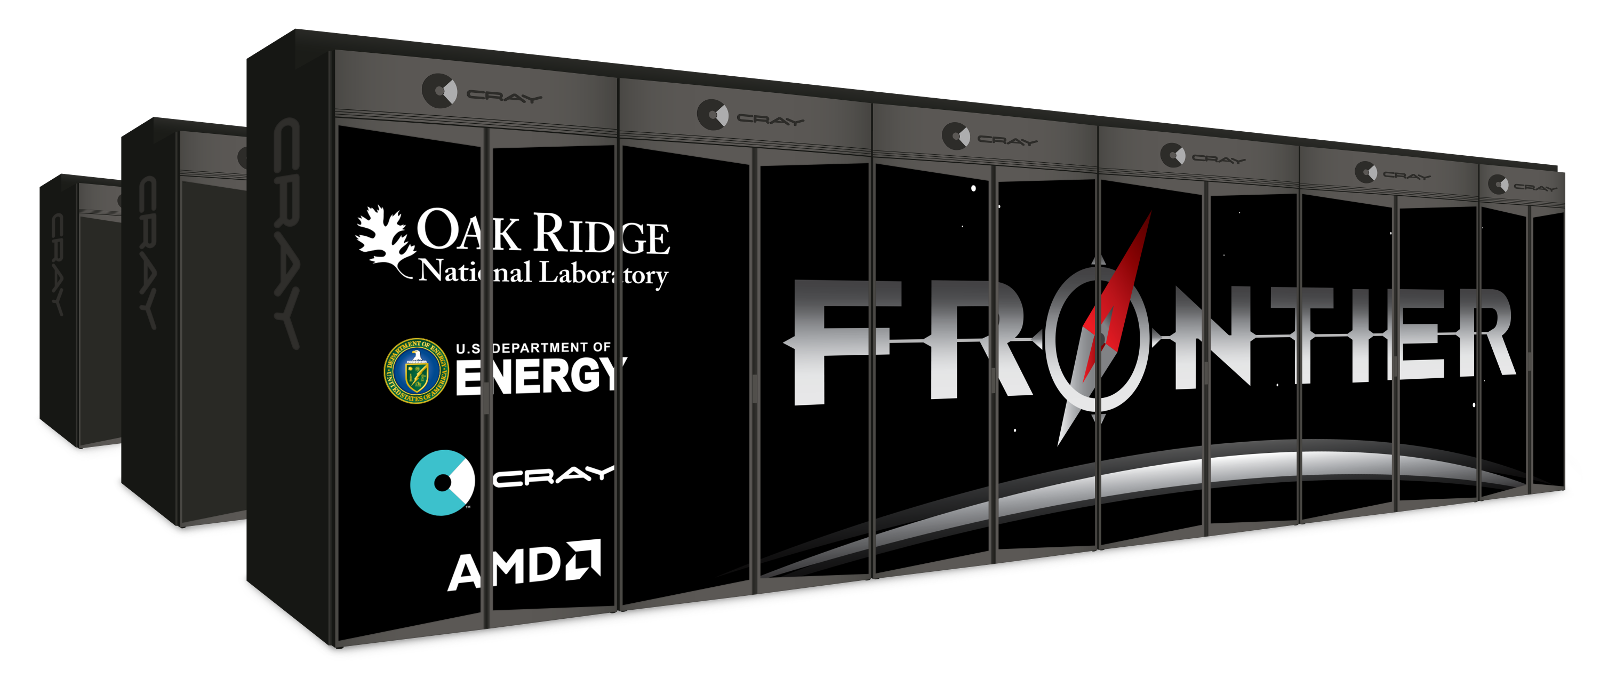
\includegraphics[width=0.75\textwidth]{./figures/frontier}
      \end{center}
    \end{column}
  \end{columns}
  \begin{columns}[T]
    \begin{column}{0.49\textwidth}
    \begin{itemize}
      \item Intel’s Xe compute architecture.
      \item $>$ 1 exaflops
    \end{itemize}
    \end{column}
    \begin{column}{0.49\textwidth}
      \begin{itemize}
        \item AMD EPYC processors and Radeon Instinct GPU
        \item 1.5 exaflops
      \end{itemize}
    \end{column}
  \end{columns}
\end{frame}

\begin{frame}
  \frametitle{Power System}
  \begin{columns}
    \begin{column}{0.45\textwidth}
      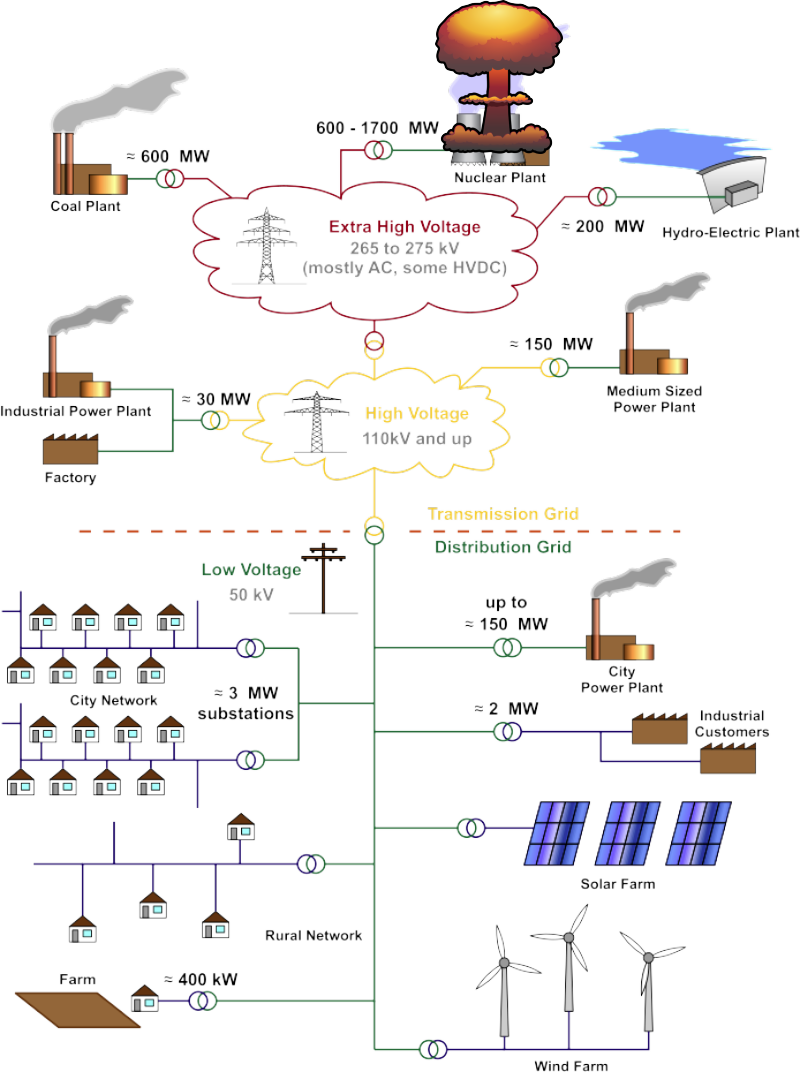
\includegraphics[width=\textwidth]{figures/slides.png}
    \end{column}
    \begin{column}{0.45\textwidth}
      \begin{center}
        % \includegraphics[width=0.8\textwidth]{figures/DampedSine.png}
      \end{center}
      \begin{itemize}
        \item Protect against contingency scenarios
        \item Demand is uncertain
        \item Generation is uncertain (solar, wind, water)
        \item Recent developments in renewable energies lead to less mass in generators decreasing inertia
        \item Less inertia worsens effects of uncertainty
      \end{itemize}
    \end{column}
  \end{columns}
\end{frame}

\begin{frame}
  \frametitle{ExaSGD: Optimizing Stochastic Grid Dynamics at Exascale
}
\begin{columns}
  \begin{column}{0.45\textwidth}
    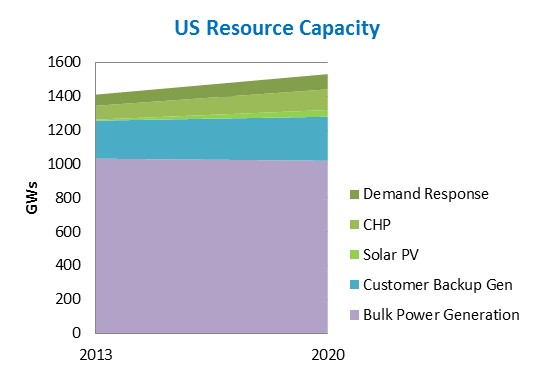
\includegraphics[width=\textwidth]{./figures/generation}
  \end{column}
  \begin{column}{0.45\textwidth}
    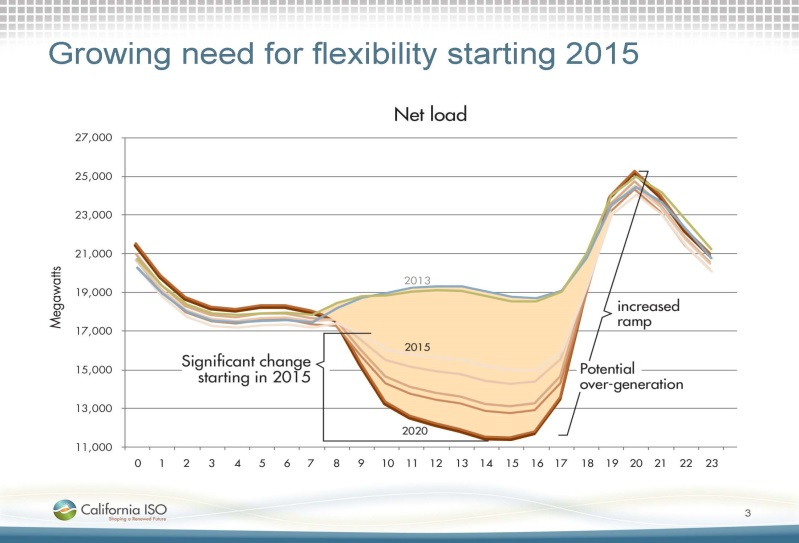
\includegraphics[width=\textwidth]{./figures/ramping}
  \end{column}
\end{columns}
  \begin{center}
      \end{center}
  {\bf Motivation:}
  \begin{itemize}
    \item More renewable energy, more uncertainty
    \item Increase in renewable energy generation ramping
  \end{itemize}
  {\bf Goals:}
  \begin{itemize}
    \item Useful long-term planning model under higher uncertainty
    \item Use AC power flow (nonlinear functions) 
    \item Efficiently leverage exascale hardware in 2021
  \end{itemize}
\end{frame}

\begin{frame}
  \frametitle{Complex Networks}
  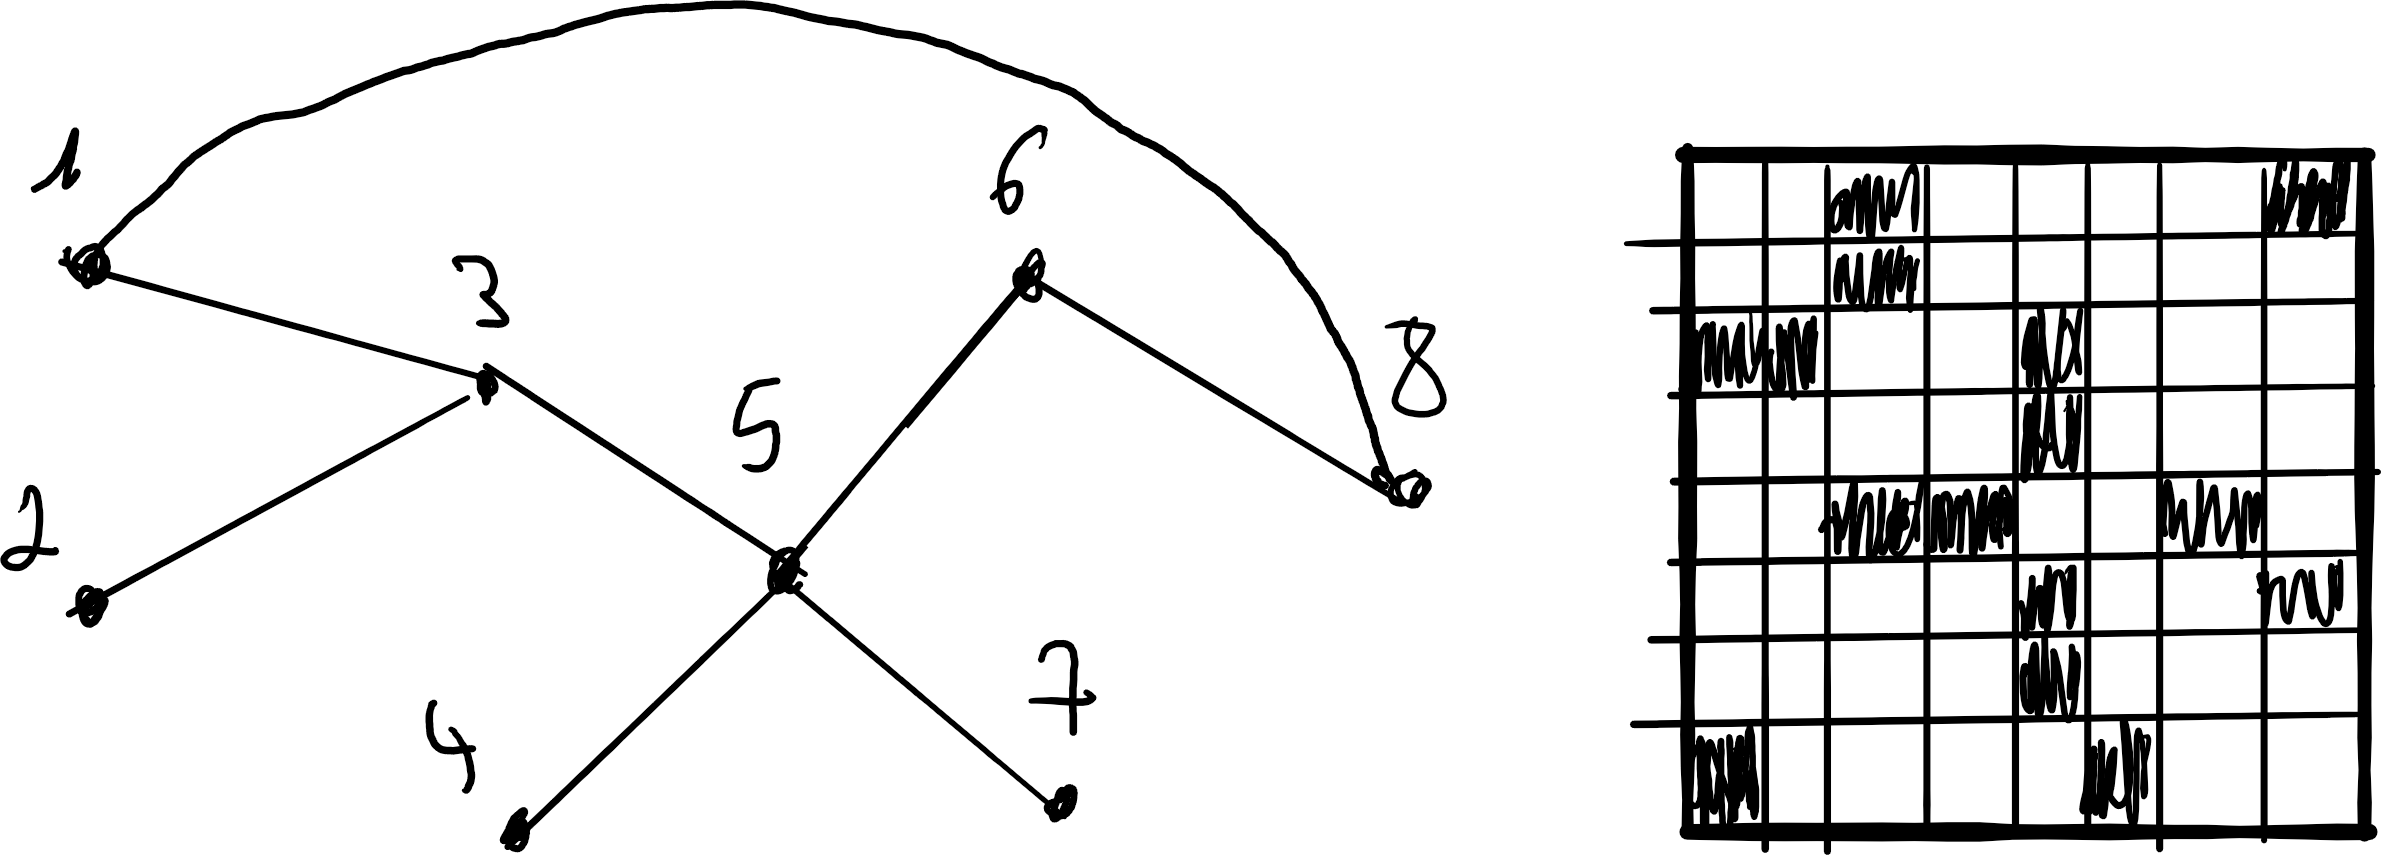
\includegraphics[width=\textwidth]{figures/complexn}
  \begin{itemize}
    \item Examples: Traffic, Internet, power grid
    \item Connection pattern is irregular but not random
    \item Different from most PDE problems (CFD)
    \item Larger cases tend to lead to ill-conditioning
  \end{itemize}
\end{frame}

\begin{frame}[fragile]
  \frametitle{Optimal Power Flow}
  \begin{itemize}
    \item {\bf Objective}
    \begin{itemize}
      \item Generation cost at generators:
      $ \minimize \sum^G_{i=1} c_i(Pg_i)$
    \end{itemize}
    \item {\bf Constraints}
    \begin{itemize}
      \item Kirchhoff's law: What flows in must flow out (nonlinear, non-convex in ACOPF)
      \begin{align*}
        V_k e^{-j\theta_k} & \sum^{N}_{m=0} (G_{km} + jB_{km})V_m e^{j\theta_m} = P - jQ,\ k = 1, \dots, N \\
        \text{where}\\
        V_k &\text{ voltage magnitude at node } k\\
        \theta &\text{ voltage angle at node } k\\
        G_{km} + jB_{km}& \text{ element of nodal admittance matrix}\\
        P, Q &\text{ net real and reactive power entering and leaving node } k
      \end{align*}
      \item Line limits \\
      $$ \theta^{min}_{nm} \leq \theta_n - \theta_m \leq \theta^{max}_{nm}$$
    \end{itemize}
  \end{itemize}
\end{frame}

\begin{frame}[fragile]
  \frametitle{Use Interior-Point for NLP}
  {\bf Solve}
  \begin{align*}
  &\minimize \phi_\mu := f(x)\\ 
  \text{with}&\\
  &g(x) \geq 0, \ i=1,\dots, m \\
  &c(x) = 0, \ j=1,\dots, l \\
  \end{align*}
  {\bf using Newton and barrier functions}
  \begin{align*}
  &\minimize \phi_\mu := f(x) - \mu \sum^m_{i=1} \ln g(x)\\ 
  \text{with}&\\
  &c(x) = 0, \ j=1,\dots, l 
  \end{align*}
  \begin{itemize}
    \item Barrier functions exacerbate ill-conditioning
  \end{itemize}
\end{frame}

\begin{frame}[fragile]
  \frametitle{Interior-Point and GPUs}
  {\bf Current State}
  \begin{itemize}
    \item Very ill-conditioned system (up $1e^{16}$)
    \item Requires sparse direct inertia revealing solver
    \item Ipopt only supports direct solver (exception: Pardiso)
    \item default MUMPS, preferred are HSL libary MA27, MA57 
    \item PIPS-NLP implements Schur complement for two-stage optimization
    \item HiOp mixed dense-sparse solver 
  \end{itemize}
\end{frame}


\begin{frame}[fragile]
  \frametitle{\sout{Optimal} Power Flow}
  \begin{itemize}
    \item {\bf \sout{Objective}}
    \begin{itemize}
      \item \sout{Generation cost at generators:
      $ \minimize \sum^G_{i=1} c_i(Pg_i)$}
    \end{itemize}
    \item {\bf Constraints}
    \begin{itemize}
      \item Kirchhoff's law: What flows in must flow out (nonlinear, non-convex in ACOPF)
      \begin{align*}
        V_k e^{-j\theta_k} & \sum^{N}_{m=0} (G_{km} + jB_{km})V_m e^{j\theta_m} = P - jQ,\ k = 1, \dots, N \\
        \text{where}\\
        V_k &\text{ voltage magnitude at node } k\\
        \theta &\text{ voltage angle at node } k\\
        G_{km} + jB_{km}& \text{ element of nodal admittance matrix}\\
        P, Q &\text{ net real and reactive power entering and leaving node } k
      \end{align*}
      \item \sout{Line limits}\\
      \sout{$ \theta^{min}_{nm} \leq \theta_n - \theta_m \leq \theta^{max}_{nm}$}
    \end{itemize}
  \end{itemize}
\end{frame}

\begin{frame}[fragile]
  \frametitle{Power Flow}
  {\bf Nonlinear equations}
  \begin{itemize}
      \item Kirchhoff's law: What flows in must flow out (nonlinear, non-convex in ACOPF)
      \begin{align*}
        V_k e^{-j\theta_k} & \sum^{N}_{m=0} (G_{km} + jB_{km})V_m e^{j\theta_m} = P - jQ,\ k = 1, \dots, N \\
        \text{where}\\
        V_k &\text{ voltage magnitude at node } k\\
        \theta &\text{ voltage angle at node } k\\
        G_{km} + jB_{km}& \text{ element of nodal admittance matrix}\\
        P, Q &\text{ net real and reactive power entering and leaving node } k
      \end{align*}
      \item Use Newton-Raphson to solve nonlinear equations
  \end{itemize}
\end{frame}

\begin{frame}
  \frametitle{Power Flow}
  {\bf Goal}
  \begin{itemize}
    \item Compute Jacobian using automatic differentiation
    \item Implement a preconditioner
    \item Implement a Krylov method
    \item No computation on the host in main loop, no data transfer
    \item All in Julia, no external calls if possible
  \end{itemize}
\end{frame}

\begin{frame}[fragile]
  \frametitle{Derivatives}
  \begin{center}
  \lstset{linewidth = \textwidth, frame=tb}
  \begin{minipage}{.3\textwidth}
    \begin{lstlisting}
    dx .= J\F
    x  .= x .- dx
    \end{lstlisting}
   \end{minipage}
  \end{center}
  \lstset{linewidth = \textwidth}
  {\bf Automatic Differentiation}
  \begin{itemize}
    \item \lstinline{F = f(x)} $\rightarrow$ \lstinline{J = jacobian(x)}
    \item Code transformation
    \item Adjoint \lstinline{adj(x, y) = (J(x))'*y)}, tangent: \lstinline{tgt(x,d) = J(x)*d} 
    \item \lstinline{size(x) >> size(F)} or \lstinline{size(x) << size(F)}
    \item number of buses $\propto$ \lstinline{size(x) = size(F)}
    \item We use \lstinline{ForwardDiff.jl}\footnote{\cite{RevelsLubinPapamarkou2016}}
  \end{itemize}
\end{frame}

\begin{frame}
  \frametitle{Jacobian Coloring}
  \begin{center}
    \begin{figure}
      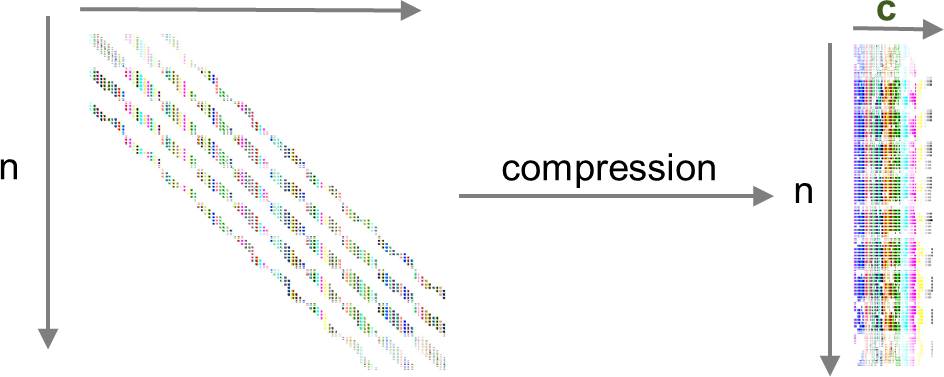
\includegraphics[width=0.65\textwidth]{figures/compression}\footnote{Thanks to Paul Hovland}
      \caption{Jacobian compression}
    \end{figure}
  \end{center}
  \begin{itemize}
    \item Sparse power grid yields very sparse Jacobian
    \item Using greedy algorithm in \lstinline{SparseDiffTools.jl}
  \end{itemize}
\end{frame}

\begin{frame}
  \frametitle{AD on GPUs in Julia}
  \begin{center}
      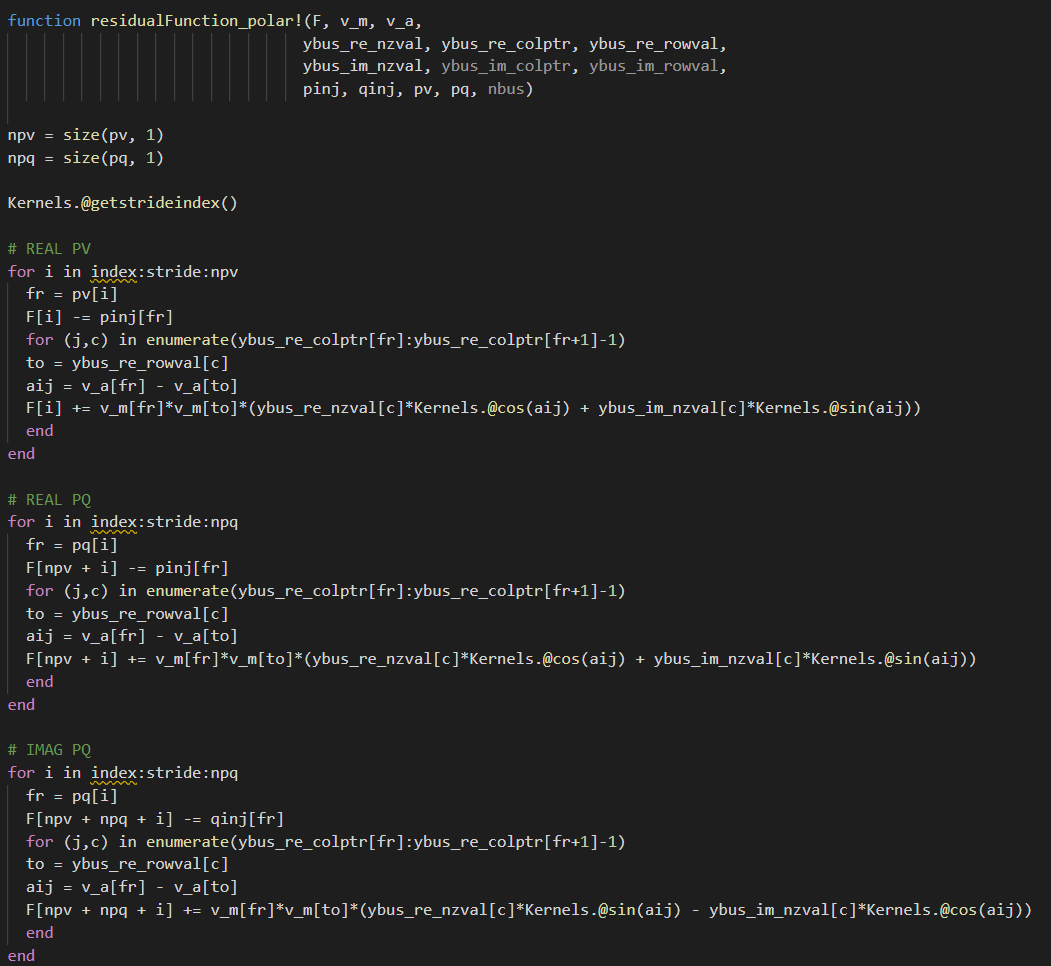
\includegraphics[width=0.75\textwidth]{figures/F}
  \end{center}
\end{frame}
\begin{frame}
  \frametitle{AD on GPUs in Julia}
  \begin{center}
    \lstinline{F = T(undef, n)}
  \end{center}
  \begin{itemize}
    \item Float vector: \lstinline{T = Vector\{Float64\}}
    \item Arbitrary precision vector: \lstinline{T = Vector\{BigFloat\}}
    \item First-order tangent: \lstinline{t1s\{N\} =  ForwardDiff.Dual\{Nothing,Float64, N\} where N}
    \item Second-order tangent: \lstinline{t2s\{M,N\} =  ForwardDiff.Dual\{Nothing,t1s\{N\}, M\} where M, N}
    \item First-order tangent vector: \lstinline{T = Vector\{t1s\{N\}\}}
    \item First-order tangent GPU vector: \lstinline{T = CuVector\{t1s\{N\}\}}
    \item Relying on \lstinline{CUDA.jl} \footnote{\cite{besard2018juliagpu}} \footnote{\cite{besard2019prototyping}}
  \end{itemize}
\end{frame}

\begin{frame}
  \frametitle{AD on GPUs in Julia}
  \begin{columns}[T]
    \begin{column}{0.35\textwidth}
      \begin{center}
        \vspace{0.2cm}
        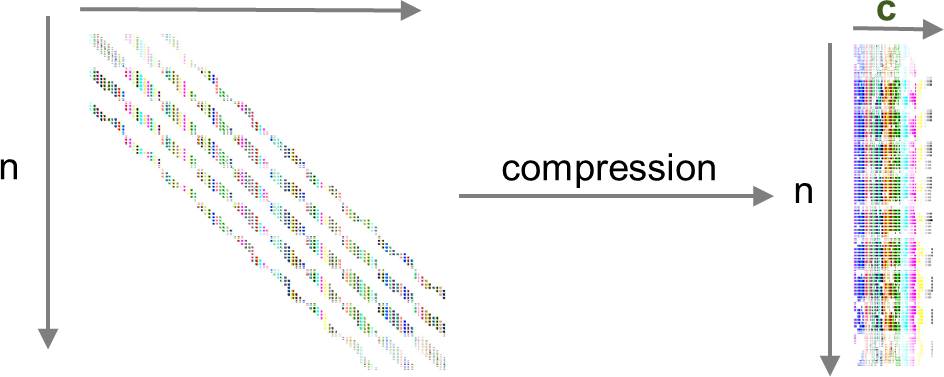
\includegraphics[width=\linewidth]{figures/compression}
      \end{center}
    \end{column}
    \begin{column}{0.6\textwidth}
      \begin{center}
        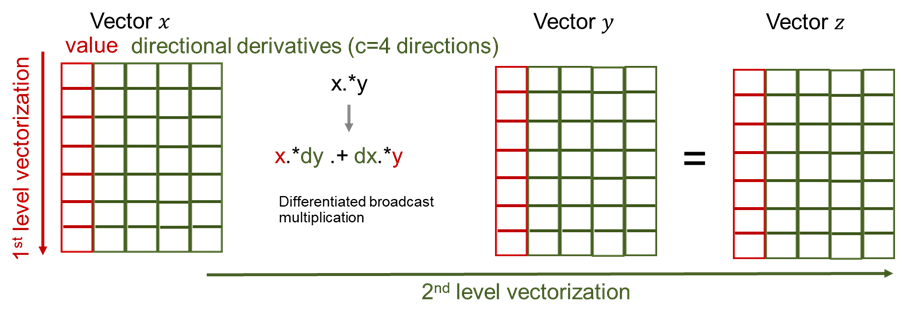
\includegraphics[width=\linewidth]{figures/simd}
      \end{center}
    \end{column}
  \end{columns}
  \begin{center}
  \end{center}
  {\bf SIMD over sparsity colors}
  \begin{itemize}
    \item Change from \lstinline{F = f(x)} to \lstinline{J = f(x)} on GPUs is a type change from \lstinline{Vector\{Float64\}} to \lstinline{CuVector\{t1s\{c\}\}}
  \end{itemize}
\end{frame}

\begin{frame}
  \frametitle{Jacobian Coloring}
  \begin{center}
    \begin{figure}
      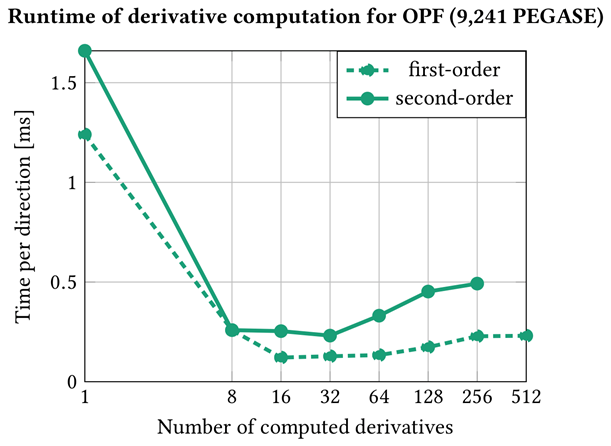
\includegraphics[width=0.35\textwidth]{figures/directionsgpu}
    \end{figure}
  \end{center}
  \begin{itemize}
    \item Sparse power grid yields very sparse Jacobian
    \item Number of colors for 9,241 bus system: 76, Hessian size: 580587x580587, compressed: 580587x76
    \item GPU strategy: Effectively SIMD parallelize over colors/directions
    \item Sweet spot on NVIDIA GV100: Chunks of 32 directions (see Figure)
    \item 0.3ms per color
    \item We don’t expect number colors to exceed 500 for final case
  \end{itemize}
\end{frame}

\begin{frame}
  \frametitle{Preconditioner}
  \begin{center}
    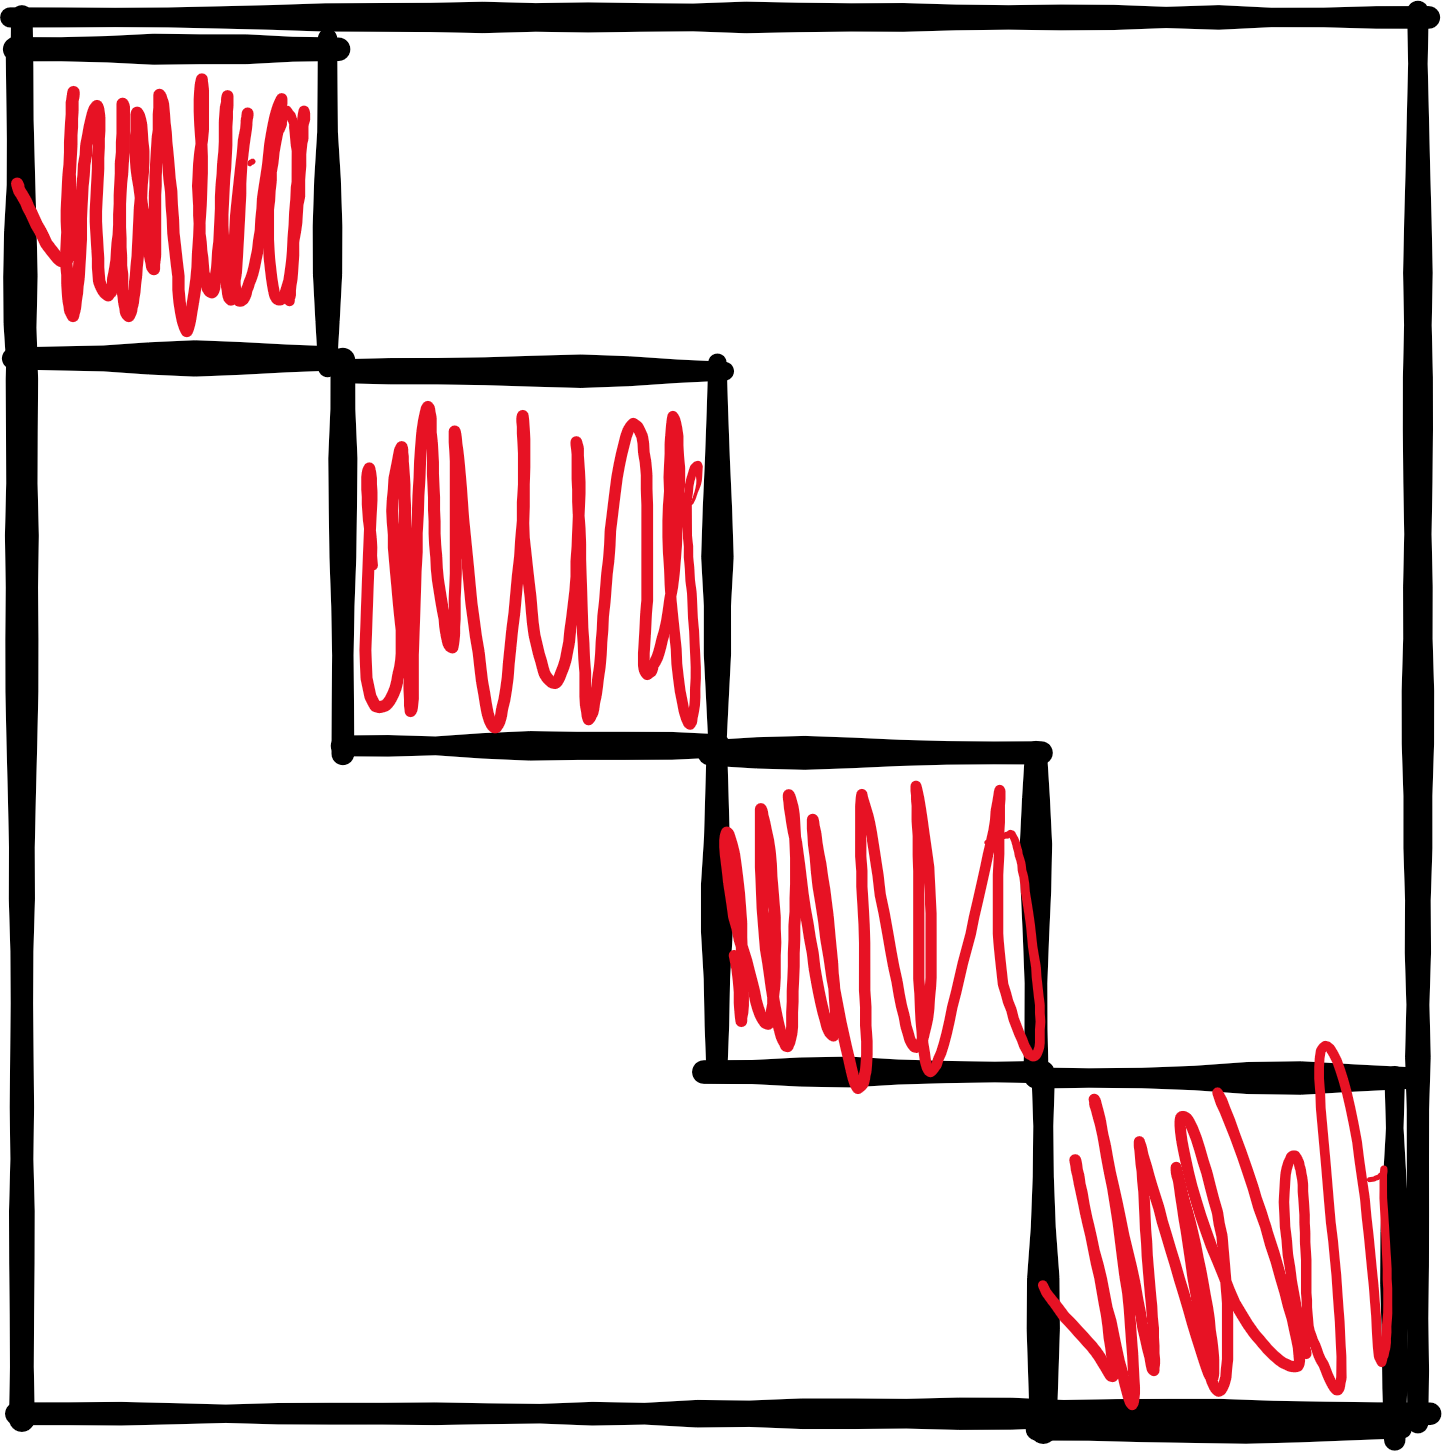
\includegraphics[width=0.25\textwidth]{figures/mpiblocks}
    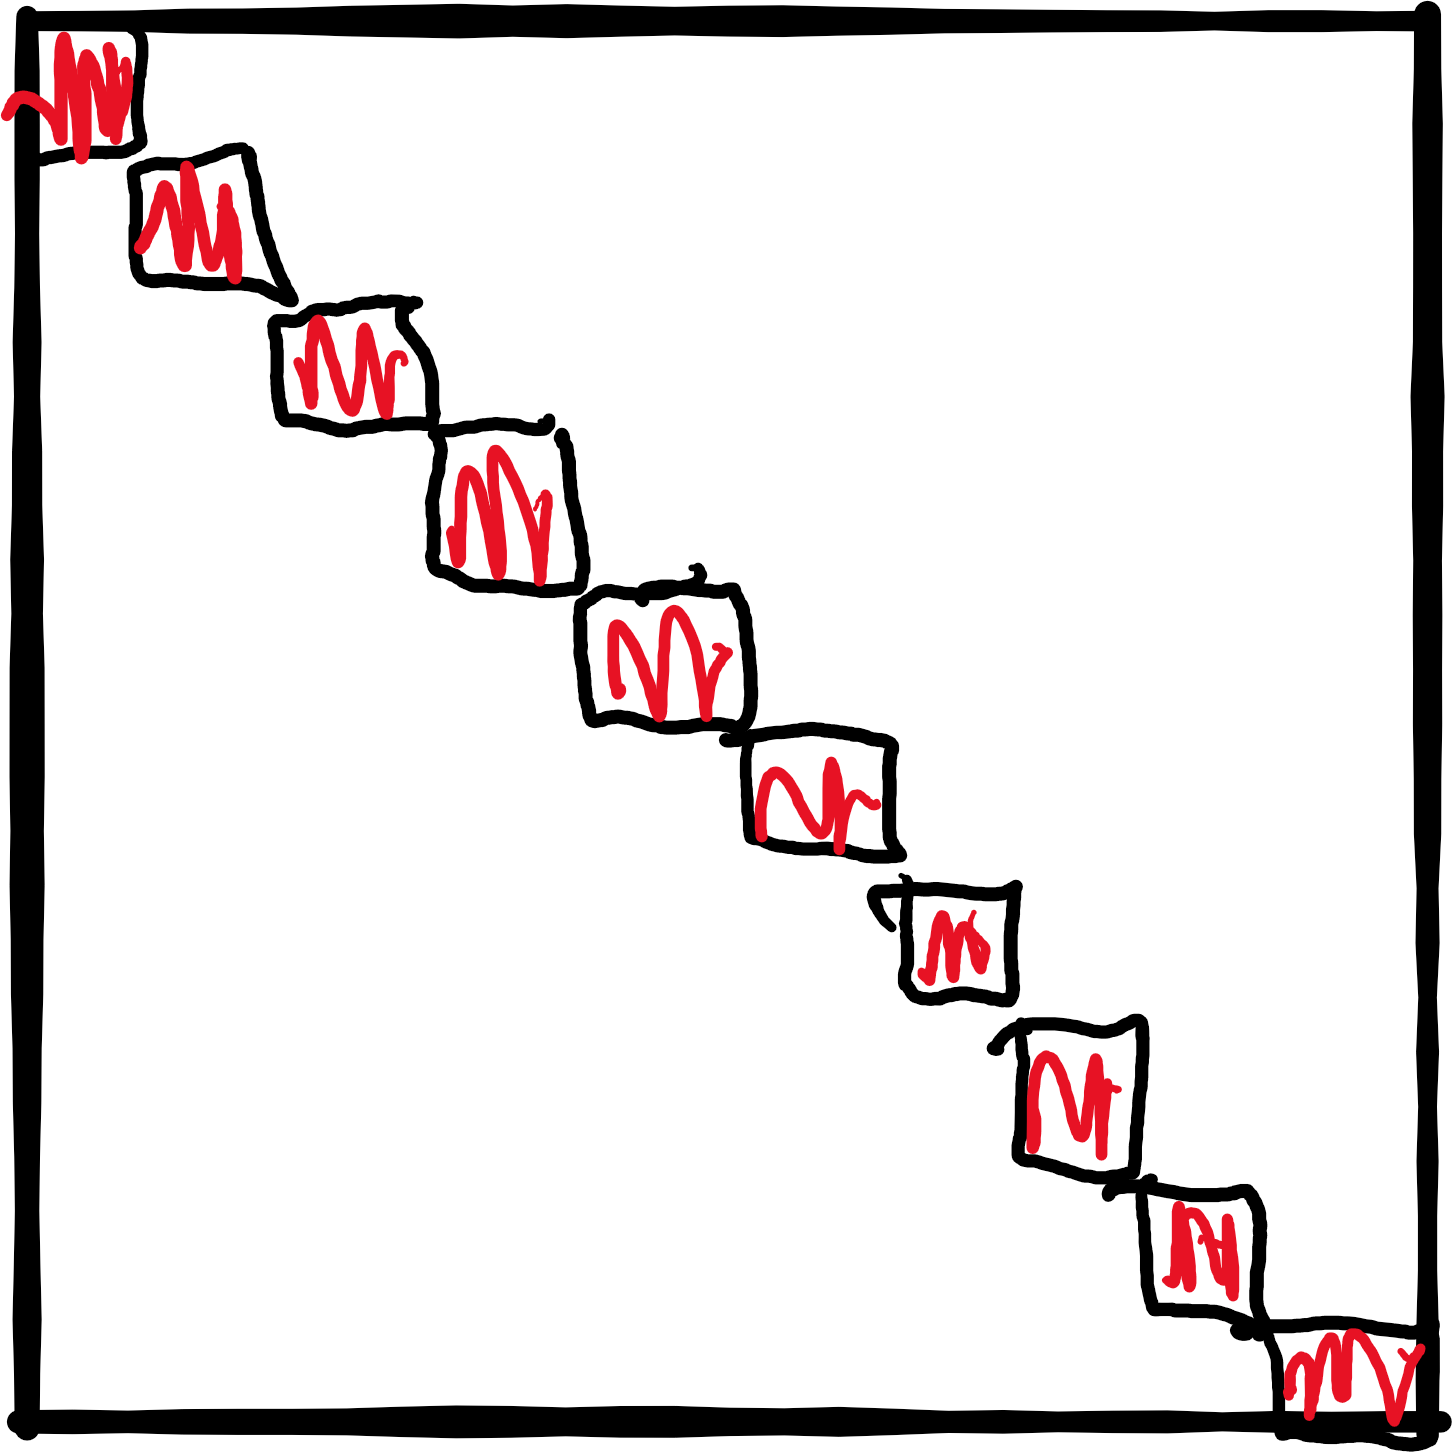
\includegraphics[width=0.25\textwidth]{figures/gpublocks}
  \end{center}
  {\bf Block-Jacobi}
  \begin{itemize}
    \item GPU implementation requires a large number of blocks
    \item PETSc per MPI process: ILU + Krylov \footnote{\cite{schwarz}} 
    \item GPU: Batch CUBLAS LU
    \item Expectation: Increase in number of blocks leads to worse preconditioner
  \end{itemize}
\end{frame}

\begin{frame}
  \frametitle{Preconditioner}
  {\bf Setup}
  \begin{itemize}
    \item Create a partitioning (METIS)
  \end{itemize}
  {\bf Iterate}
  \begin{itemize}
    \item Update P
    \begin{enumerate}
      \item Read dense compressed Jacobian into dense Jacobi blocks
      \item Batch inversion
      \item Update sparse matrix P from dense Jacobi blocks
    \end{enumerate}
  \end{itemize}
  {\bf Code size}
  \begin{itemize}
    \item 200 lines of code for BOTH CPU and GPU implementation
  \end{itemize}
\end{frame}

\begin{frame}
  \frametitle{Preconditioner}
  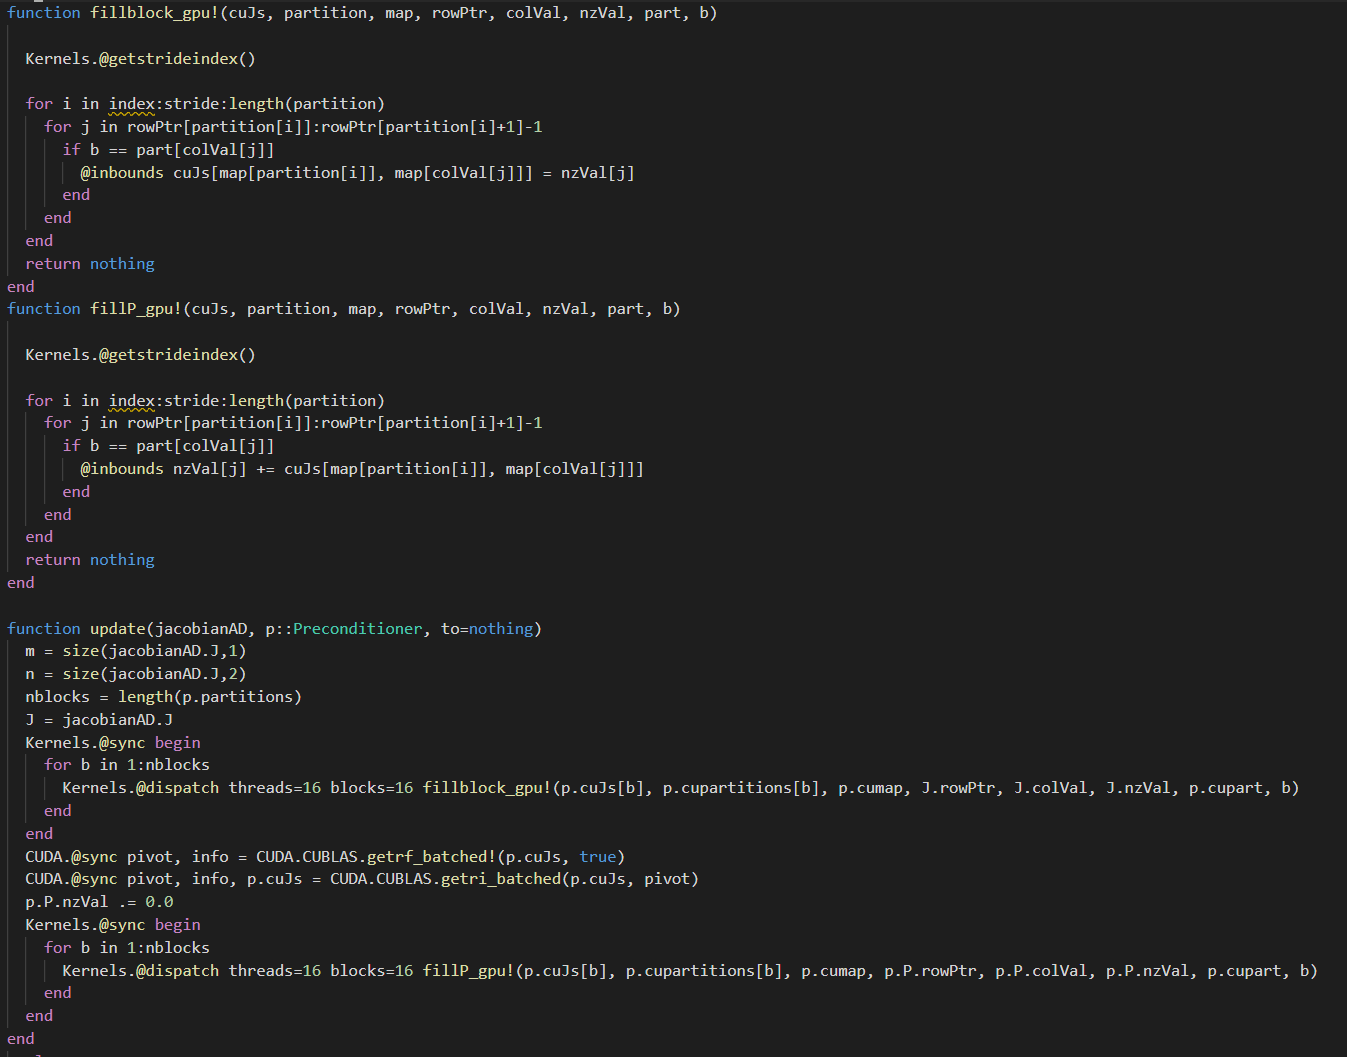
\includegraphics[width=0.95\textwidth]{figures/preconditioner}
\end{frame}

\begin{frame}
  \frametitle{Linear solver}
  {\bf Tour de Solvers}
  \begin{itemize}
    \item Indefinite sparse direct solvers: MA27, MA57, MUMPS, SQPR, CUSOLVER, SPRAL SSIDS
    \item Indefinite dense direct solvers: BLAS, CUBLAS
    \item Sparse positive definite solvers: CHOLMOD, SPRAL SSIDS
    \item Iterative solvers: \lstinline{IterativeSolvers.jl}, \lstinline{Krylov.jl} 
    \item GMRES and BiCGSTAB \footnote{\cite{bicgstabVorst}} \footnote{\cite{sleijpen1993bicgstab}}
  \end{itemize}
\end{frame}

\begin{frame}[fragile]
  \frametitle{Linear Solver}
  \begin{center}
   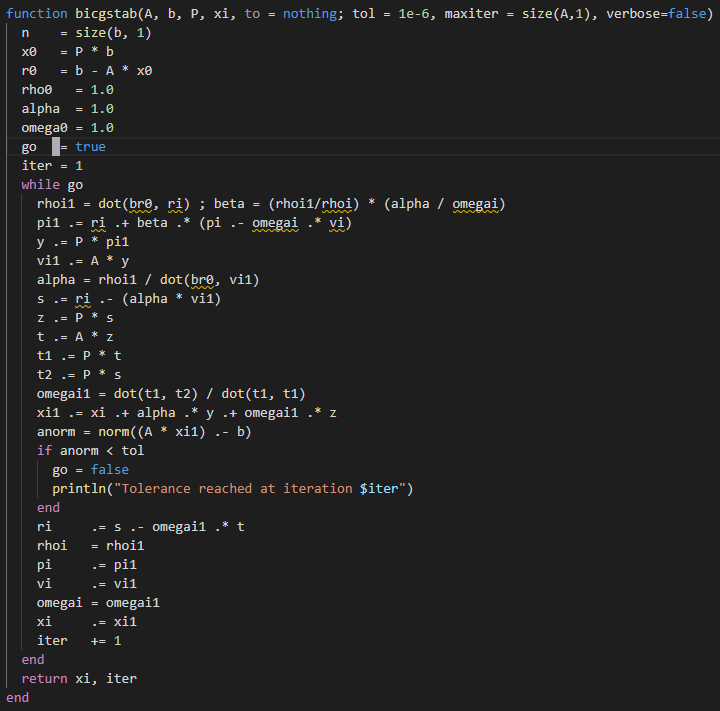
\includegraphics[width=0.7\textwidth]{figures/bicgstab.png}
  \end{center}
\end{frame}

\begin{frame}[fragile]
  \frametitle{ExaPF.jl}
  \begin{lstlisting}
    pkg> instantiate
    julia> target = "cuda" 
    julia> include("examples/pf.jl") 
    julia> datafile = "test/case14.raw"
    julia> sol, conv, res = pf(datafile, 8, "bicgstab") # slow
    julia> sol, conv, res = pf(datafile, 8, "bicgstab")
  \end{lstlisting}
  \begin{itemize}
    \item \url{https://exanauts.github.io/}
    \item Julia for Summit builds
    \item Other research software
    \item \url{https://github.com/exanauts/ExaPF.jl}
  \end{itemize}
\end{frame}

\begin{frame}[fragile]
  \frametitle{ExaPF.jl}
  {\bf 30,000 bus system}
  \begin{lstlisting}
    julia> datafile = "GO-Data/.../Network_30R-025/.../case.raw"
    julia> sol, conv, res = pf(datafile, 1000, "bicgstab")
  \end{lstlisting}
  \begin{itemize}
    \item \lstinline{size(J)} = 57,721 $\times$ 57,721 
    \item Block Jacobi size: 59 $\times$ 59 $\approx$ 25 MB
    \item Total GPU memory usage: 5 GB
    \item Number of Jacobian colors: 29
    \item 4 Newton iterations with $tol = 1e^{-6}$, total BiCGSTAB iterations: 3,752 
  \end{itemize}
\end{frame}

\begin{frame}[fragile]
  \frametitle{ExaPF.jl}
  {\bf 30,000 bus system}
  \begin{itemize}
    \item \lstinline{size(J)} = 57,721 $\times$ 57,721 
    \item Block Jacobi size: 59 $\times$ 59 $\approx$ 25 MB
    \item Total GPU memory usage: 5 GB
    \item Number of Jacobian colors: 29
    \item 4 Newton iterations with $tol = 1e^{-6}$, total BiCGSTAB iterations: 3,752 
  \end{itemize}
  \begin{center}
   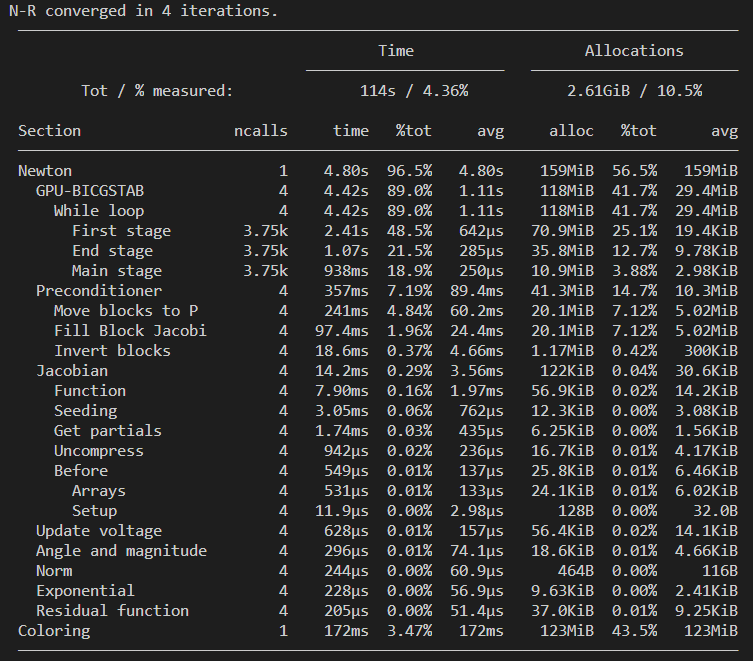
\includegraphics[width=0.45\textwidth]{figures/timings}
  \end{center}
\end{frame}

\begin{frame}
  \frametitle{ExaPF.jl}
  {\bf Context}
  \begin{itemize}
    \item CUSOLVE: 10s 
    \item Sparse Julia \lstinline{J\F} (probably UMFPACK): 3.49s 
    \item Block Jacobi + BiCGSTAB in ExaPF.jl
    \begin{itemize}
      \item Jacobian: 14.2 ms
      \item Preconditioner: 357 ms
      \item BiCGSTAB: 4.42s
      \item Total: 4.8s
    \end{itemize}
  \end{itemize}
\end{frame}

\begin{frame}[fragile]
  \frametitle{ExaPF.jl}
  {\bf BiCGSTAB iterations with decreasing block size}
  \begin{center}
   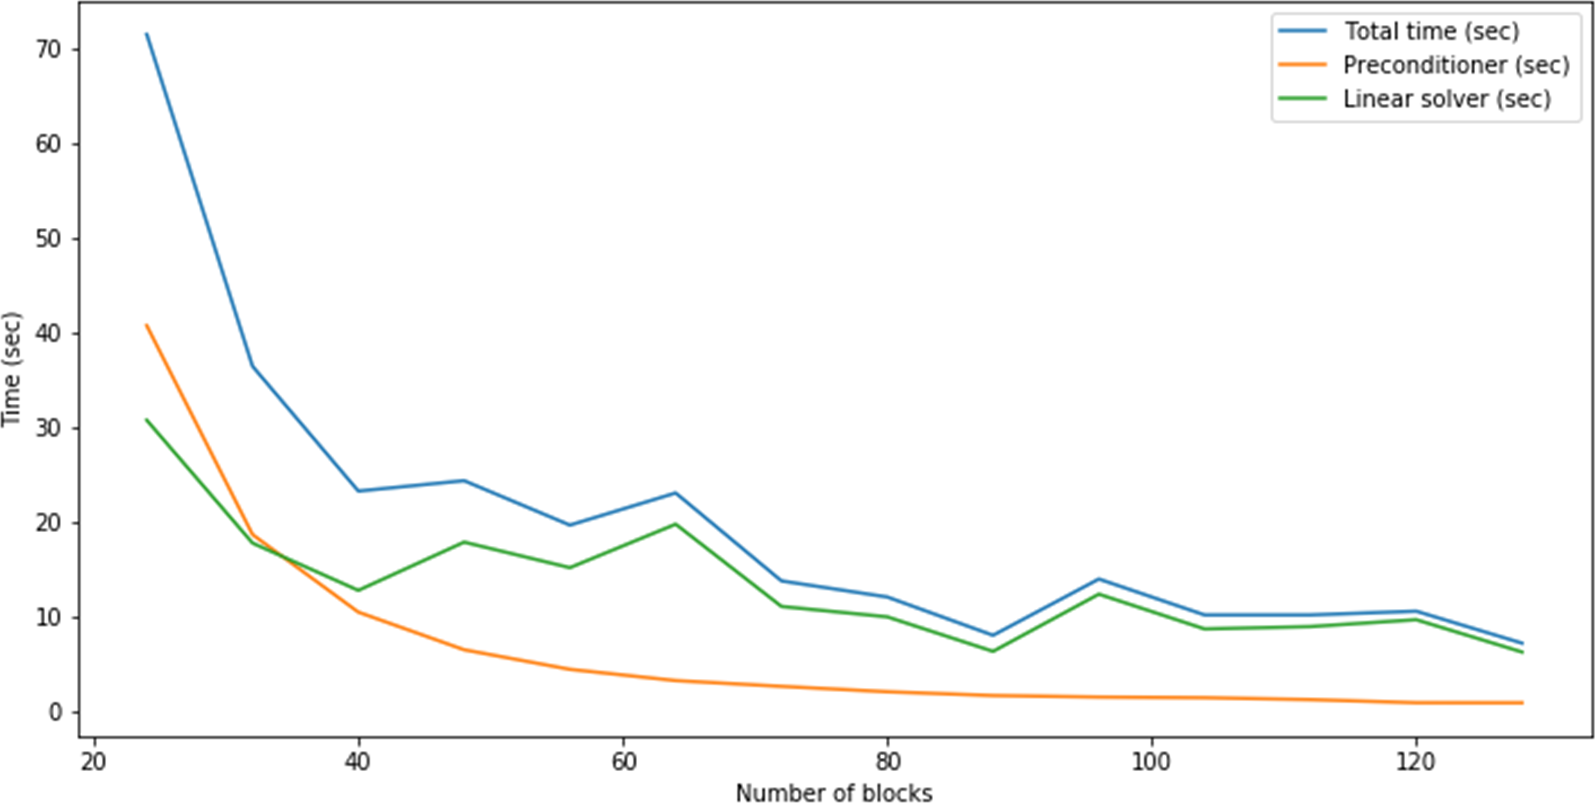
\includegraphics[width=0.45\textwidth]{figures/blocks}
   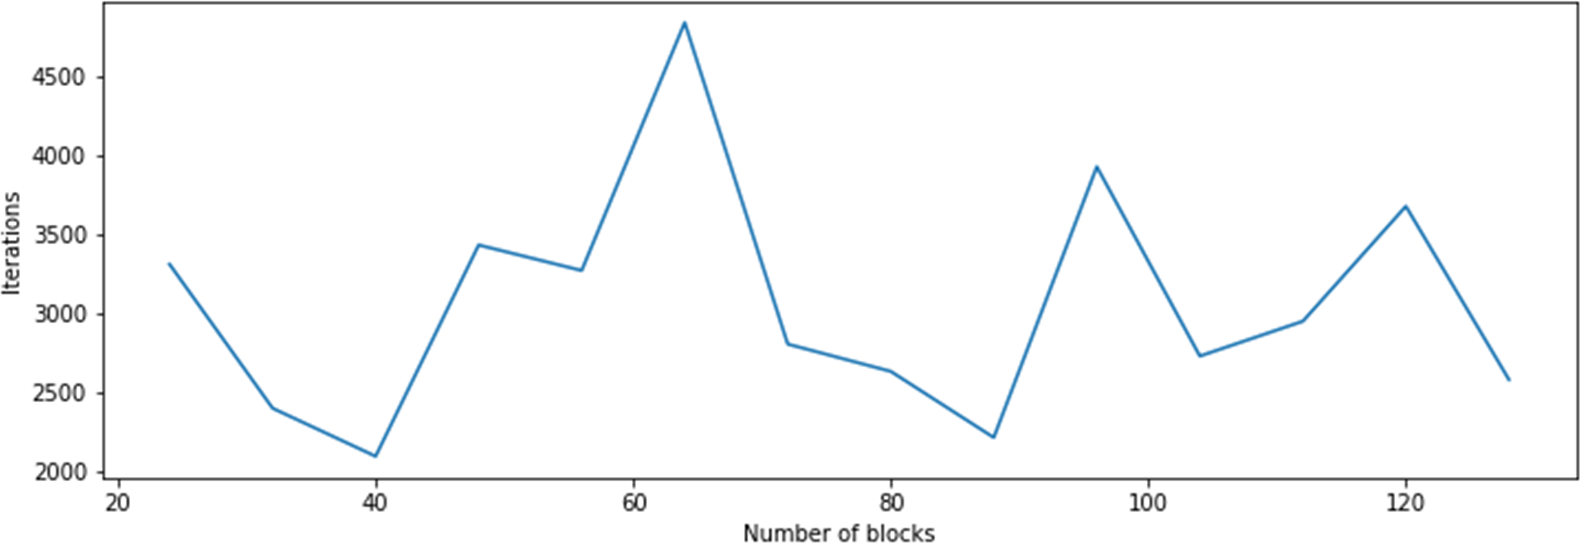
\includegraphics[width=0.45\textwidth]{figures/bicgstabiter}
  \end{center}
  \begin{itemize}
    \item Smaller blocks decrease memory footprint by $\frac{1}{n}$ 
    \item Smaller blocks speed up application of preconditioner in BiCGSTAB $P * x$
    \item BiCGSTAB unimpressed by smaller block sizes, however FAILS to converge without preconditioner
    \item Block Jacobi size: 464 $\times$ 464 $\approx$ 200 MB
    \item 4 Newton iterations with $tol = 1e^{-6}$
  \end{itemize}
\end{frame}

\begin{frame}
  \frametitle{Conclusions}
  \begin{itemize}
    \item Much harder systems for OPF with inequality constraints
    \item Other GPU first preconditioners
    \item Rapid prototyping in Julia is fast
    \item SIMD modeling framework
    \item Reduced gradient method for OPF
  \end{itemize}
\end{frame}

\begin{frame}[noframenumbering,plain,allowframebreaks]{References}
    \printbibliography[heading=none]
\end{frame}




%\bibliographystyle{unsrtnat}
\end{document}

